\begin{solution}{hard}
From idea 19 we conclude that the shape of the cross-section of the meniscus is identical to the cross-section of the pool of liquid laying on the desk (cf. problem 29). This is because on each point of the surface, we have the surface tension and gauge pressure cancelling out each other to result into the same type of the surface except inverted as shown in the picture below (the result is also rather intuitive if you think about it). From fact 17 we conclude that we only have to look at half of the height of the pool of liquid since in cylindrical geometry the pressure becomes halved.
\begin{center}
    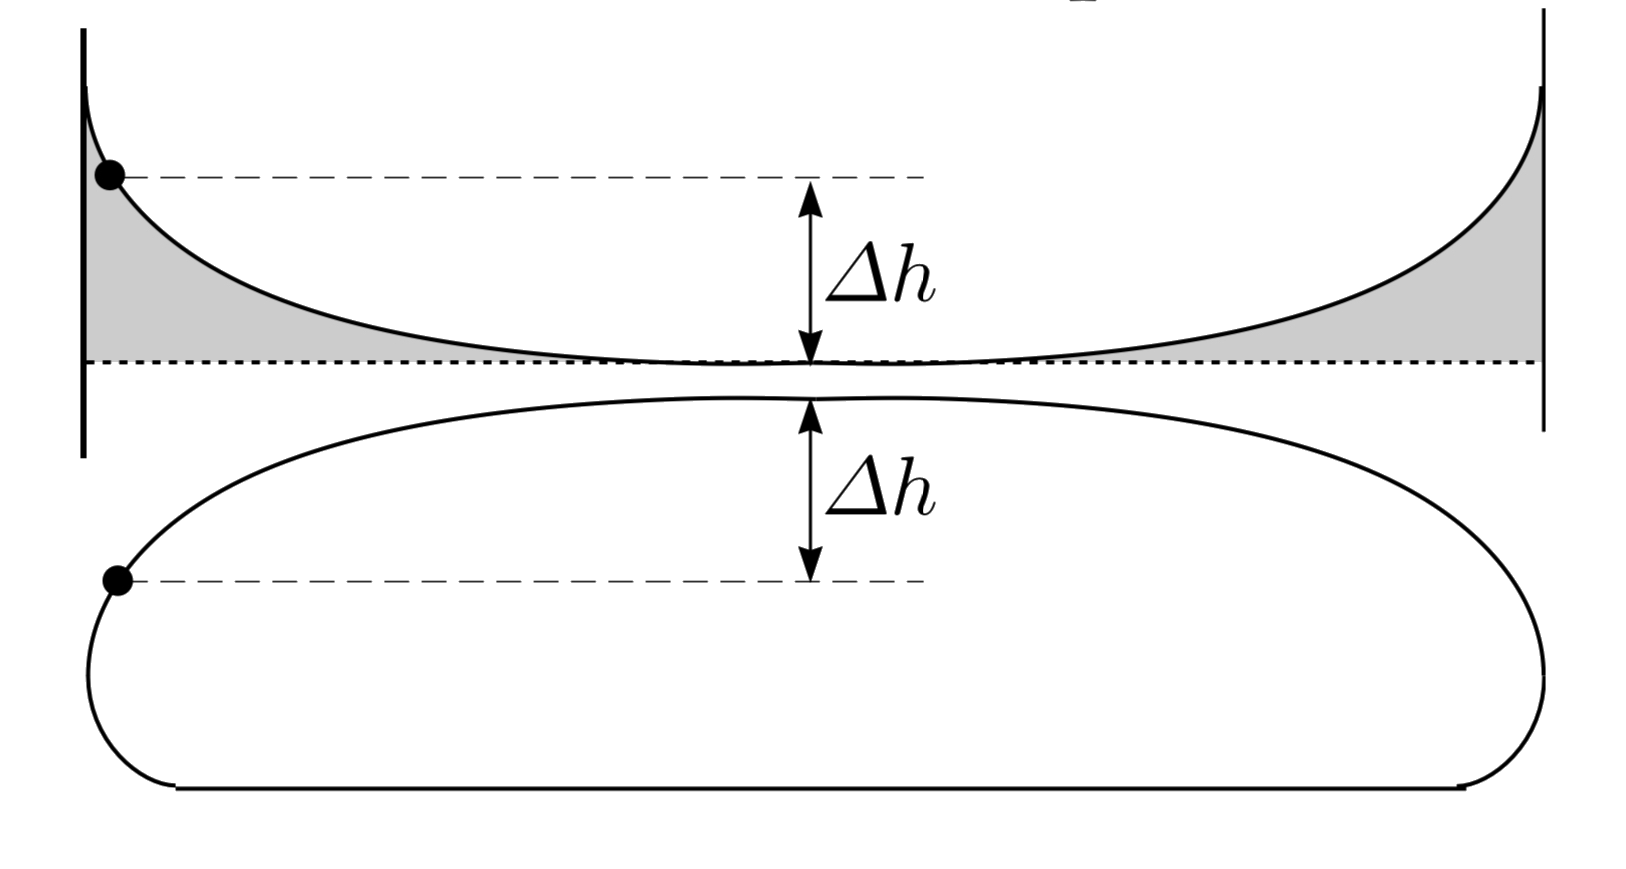
\includegraphics[width=10cm]{pr30.png}
\end{center}
From problem 29, we can conclude that the height is given by 
\[h = \sqrt{\frac{2\sigma}{\rho g} (1 -\cos\theta)}.\]
Since the contact angle is $180^{\circ}$, we have that $\cos 180^{\circ} = -1\implies h = 2\sqrt{\frac{\sigma}{\rho g}}$ we can then find that the height of the meniscus is half of this or in other words $h_m = \boxed{\sqrt{\frac{\sigma}{\rho g}}}$.
\end{solution}